% CVPR 2025 Paper Template; see https://github.com/cvpr-org/author-kit

\documentclass[10pt,twocolumn,letterpaper]{article}

%%%%%%%%% PAPER TYPE  - PLEASE UPDATE FOR FINAL VERSION
% \usepackage{cvpr}              % To produce the CAMERA-READY version
\usepackage[review]{cvpr}      % To produce the REVIEW version
% \usepackage[pagenumbers]{cvpr} % To force page numbers, e.g. for an arXiv version

% Import additional packages in the preamble file, before hyperref
%
% --- inline annotations
%
\newcommand{\red}[1]{{\color{red}#1}}
\newcommand{\todo}[1]{{\color{red}#1}}
\newcommand{\TODO}[1]{\textbf{\color{red}[TODO: #1]}}
% --- disable by uncommenting  
% \renewcommand{\TODO}[1]{}
% \renewcommand{\todo}[1]{#1}


\usepackage{algorithm}
\usepackage{algorithmic}

% It is strongly recommended to use hyperref, especially for the review version.
% hyperref with option pagebackref eases the reviewers' job.
% Please disable hyperref *only* if you encounter grave issues, 
% e.g. with the file validation for the camera-ready version.
%
% If you comment hyperref and then uncomment it, you should delete *.aux before re-running LaTeX.
% (Or just hit 'q' on the first LaTeX run, let it finish, and you should be clear).
\definecolor{cvprblue}{rgb}{0.21,0.49,0.74}
\usepackage[pagebackref,breaklinks,colorlinks,allcolors=cvprblue]{hyperref}

%%%%%%%%% PAPER ID  - PLEASE UPDATE
\def\paperID{9970} % *** Enter the Paper ID here
\def\confName{CVPR}
\def\confYear{2025}

%%%%%%%%% TITLE - PLEASE UPDATE
\title{Towards Efficient and Accurate Spiking Neural Networks via Adaptive Bit Allocation}

%%%%%%%%% AUTHORS - PLEASE UPDATE
\author{First Author\\
Institution1\\
Institution1 address\\
{\tt\small firstauthor@i1.org}
% For a paper whose authors are all at the same institution,
% omit the following lines up until the closing ``}''.
% Additional authors and addresses can be added with ``\and'',
% just like the second author.
% To save space, use either the email address or home page, not both
\and
Second Author\\
Institution2\\
First line of institution2 address\\
{\tt\small secondauthor@i2.org}
}
% my env
\usepackage{booktabs}
\usepackage{threeparttable}
\usepackage{adjustbox}
\usepackage{multirow} % Required for multirows 
\usepackage{amsmath}
\usepackage[table,xcdraw]{xcolor}
\usepackage[normalem]{ulem}
\useunder{\uline}{\ul}{}

\newtheorem{theorem}{Theorem}
\newtheorem{lemma}{Lemma}
\newtheorem{proof}{Proof}

\begin{document}
\maketitle
% \input{sec/0_abstract}    
% \input{sec/1_intro}
% \input{sec/2_formatting}
% \input{sec/3_finalcopy}


\begin{abstract}
Multi-bit spiking neural networks (SNNs) have recently become a heated research spot, persuing energy-efficient and high-accurate AI. 
However, with more bits involved, the memory and computation requirements grow so significantly that the substantial performance lift become out of proportion. 
Based on the insight that different layers demonstrate different importance and extra bits could be wasted and interfering, this paper presents an adaptive bit allocation method for direct-trained SNNs, advancing efficiency and accuracy. 
Specifically, we parametrize the bit widths of weights, spikes and temporal lengths, and make them learnable and controllable through gradients. 
Tackling rising issues  due to changeable bits and temporal lengths, we propose 
the refined spiking neuron that can handle different temporal lengths, enable the derivation of gradients for temporal lengths, and suits spike quantization better. In addition, we theoretically formulate the step-size mismatch problem of  learnable widths, which may incur severe inference errors to SNN, and accordingly propose the step-size renew mechanism to alleviate this issue. 
Extensive experiments on a variety of datasets, including the static CIFAR and ImageNet and the dynamic CIFAR-DVS, demonstrate that our method can reduce the memory and computation cost by a significant margin, while achieving higher classification accuracy. Particularly, our SEWResNet-34 with 15.4 bit budgets can achieve the advanced 72.82\% top-1 accuracy on ImageNet.
This project will be open-sourced.


\end{abstract}
\section{Introduction}
\label{sec:intro}






\begin{figure}[t]
  \centering
  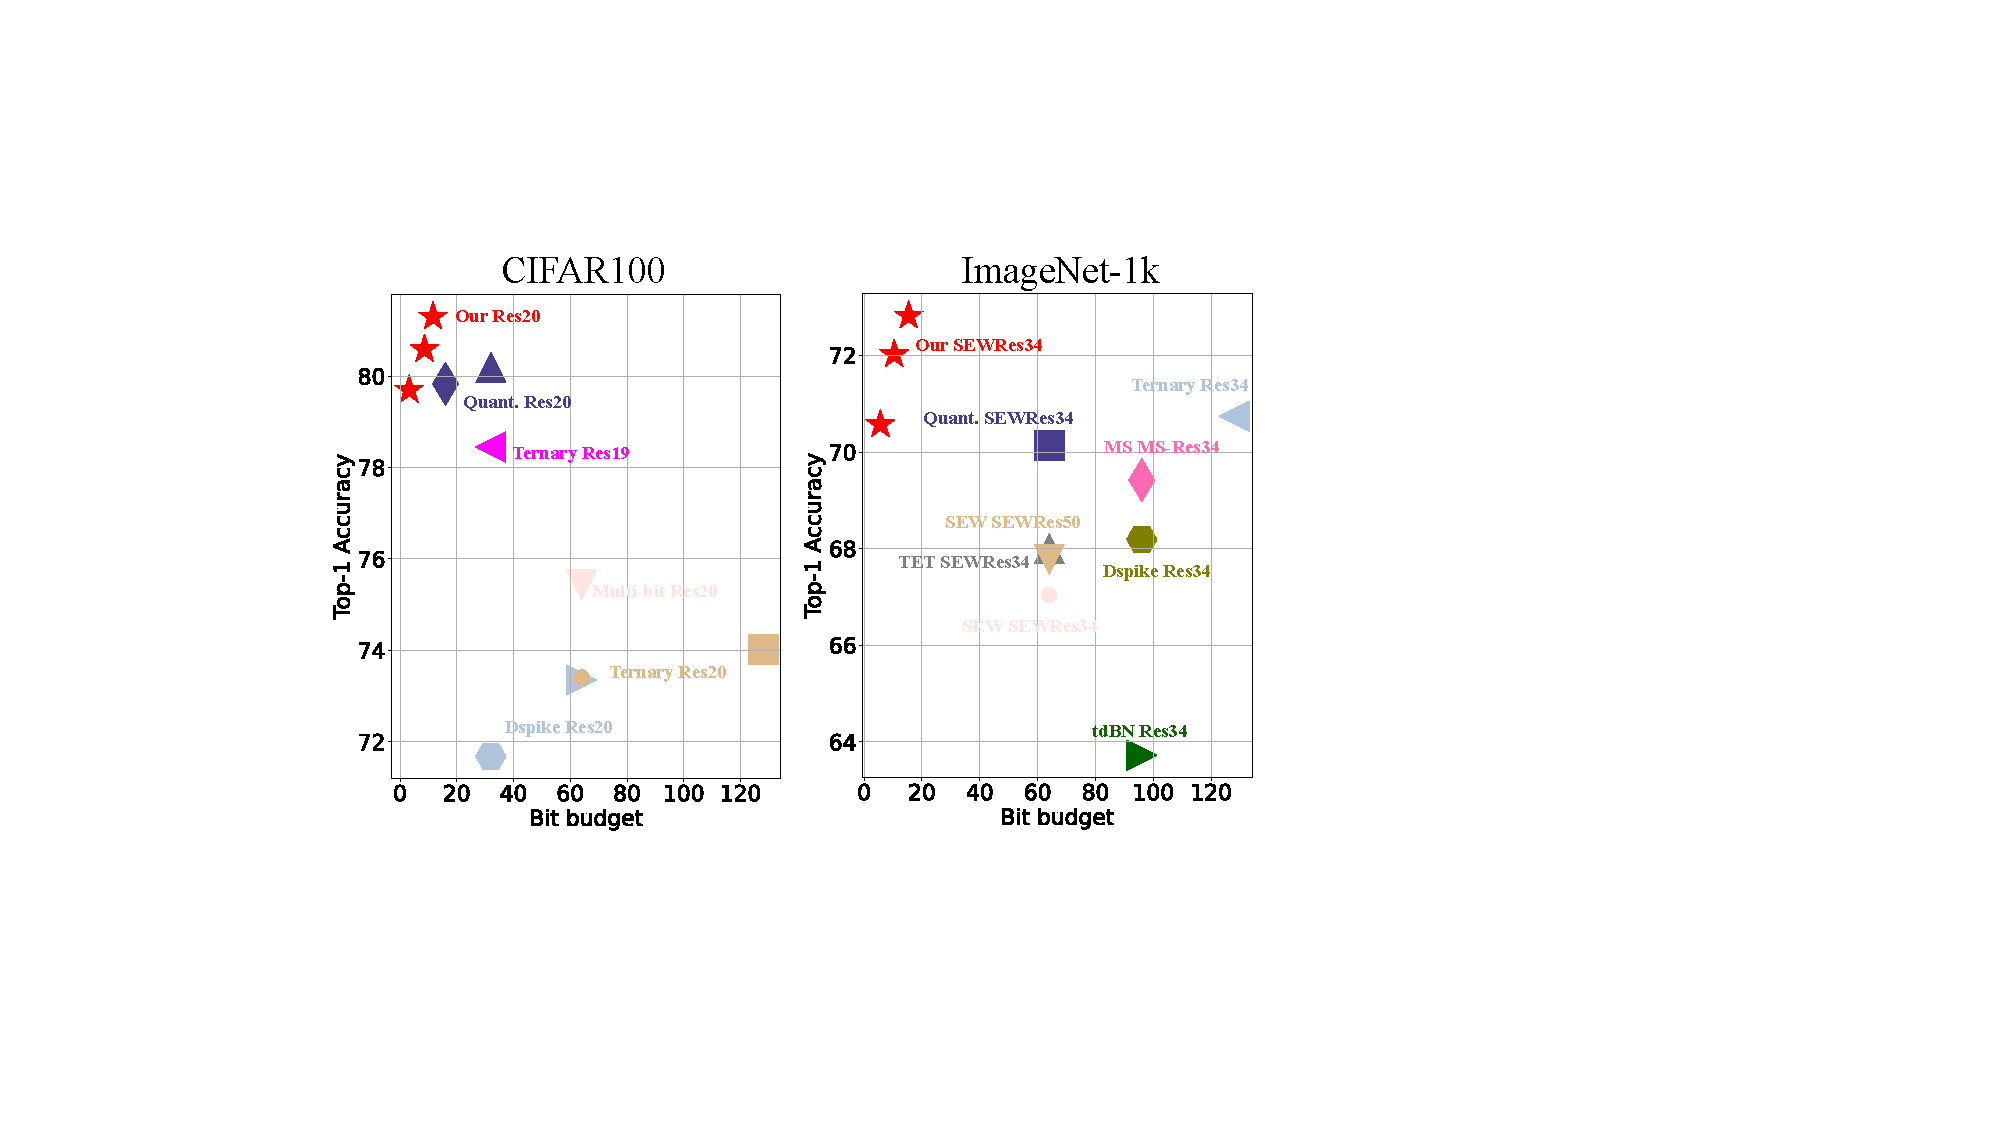
\includegraphics[width= 8cm]{figs/intro.pdf}
  \caption{Comparisons with other advanced SNNs using ResNet-based architectures on CIFAR100 and ImageNet-1k. Our models maintain the same level of model size as our baselines.}
  \label{fig:intro}
\end{figure}


Spiking neural networks (SNNs) are considered the third generation of neural networks \cite{maass1997networks}. The essential uniqueness of SNN is its activation unit, \ie, spiking neuron, that transfers the float value into binary spike, thus making the matrix operations, \eg, convolution, conducted in a multiplication-free way \cite{fang2021deep}. Similar to binary neural networks (BNN), binary feature maps (spikes) result in a reduction in spatial representation ability, making it challenging to process information-dense data and resulting in lower model accuracy \cite{zhu2019binary, meng2022training,zhou2022spikformer}.

Such being the case, multi-bit spiking neural networks have recently arisen as a promising approach to improving such inadequate informational scope \cite{guo2024ternary, xing2024spikellm,xing2024spikelm,xiao2024multi}. As the name suggests, multi-bit SNNs introduce more bits to represent the original binary spike and devote more addition operations to process the matrix multiplication. Prior arts successfully incorporate this mechanism to improve accuracy, while most of them neglect the actual memory and computation overhead as pointed out by  \cite{shen2024conventional}.
For example, a layer with less representation ability but assigned with high bit width would incur memory and computation waste and interfere the model inference \cite{dong2019hawq,Chen_2021_ICCV}. 
It desperately comes to the 
question: \emph{could we boost the performance of SNNs while maintain a constrained low-level memory and  computation overhead?} 

\begin{figure*}[t]
  \centering
  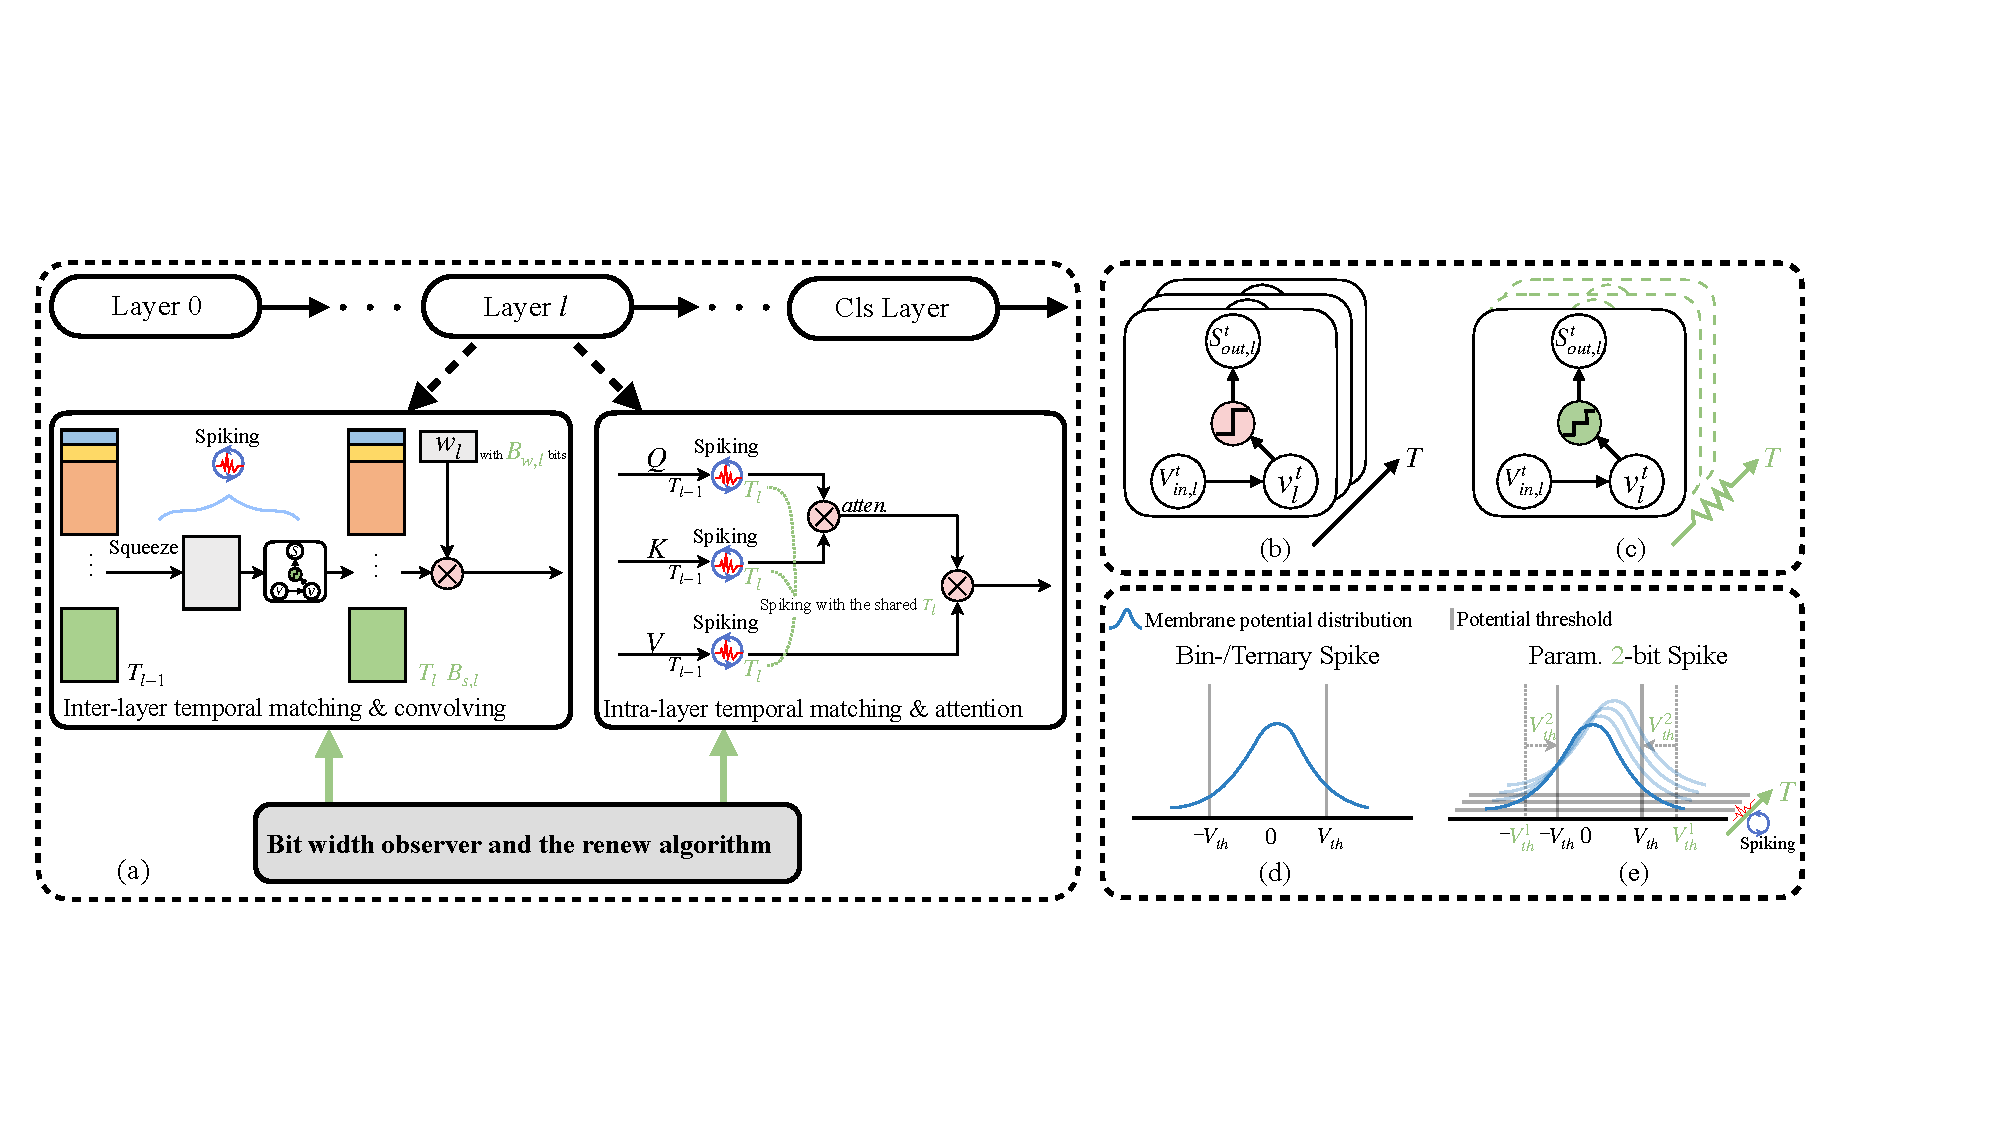
\includegraphics[width= 16cm]{figs/overview.pdf}
  \caption{Overview of the  proposed  bit allocation method. Green notations denote the parametrized constants. \textbf{(a)} Adaptive-bit-allocation training pipline, where the bit widths $T_l$, $B_{s,l}$, and $B_{w,l}$ are made learnable. $T_l$ is matched inter- and intra-layer to ensure the sufficient and fluent dataflow. The step-size renew mechanism is also proposed to alleviate the step-size mismatch issue. \textbf{(b)} and \textbf{(d)} depict the neuron formulation and the potential division of the previous binary and ternary spiking neuron, respectively. \textbf{(c)} and \textbf{(e)} depict our refined multi-bit spiking neuron, where the temporal length $T_l$ is layer-wise learnable and a shift $V^2_{th,l}$ is added to the potential threshold $V^1_{th,l}$. }
  \label{fig:overview}
\end{figure*}
In this paper, we investigate the adaptive bit allocation to answer this question. Specifically, we incorporate the pragmatic concept “Bit Budget” proposed by  \cite{shen2024conventional} and parametrize the three fundamental elements of bit budget: the bit widths of weights, spikes and temporal lengths, which also means the whole model is quantized. Thus, we can estimate the accurate model memory and computation by averaged bit width (Bit budget) and combined addition operation (S-ACE).
We then solve those non-differentiable terms to make these bit widths become learnable and can be optimized by the task loss signal. 
To constrain the changing of bit widths, we explicitly set bit bounds and implicitly design the bit width  loss to make the bit widths converge to the target widths correctly.

However, the special temporal dimension of SNN would pose new challenges. Firstly, the temporal dimension originally does not get involved in the forward pass, thus 
failing to get gradients for optimization. 
Secondly, previous multi-bit spiking neuron is designed and tuned chaotically, showing less friendliness to quantization. Thirdly, the potential step-size mismatch issue of learnable bit widths may become more severe as the temporal dimension
would consecutively use a wrong step size.
As illustrated in  \cref{fig:overview}, we first refine the spiking neuron, making it able to tackle temporal length mismatch inter- and intra-layer caused by changeable temporal length, and reducing quantization error via better formulations and potential divisions.
Then, we theoretically formulate the quantization step-size mismatch issue, where SNN would suffer a more severe offset that accumulates along the temporal dimension. Accordingly,
we propose the step-size renew mechanism, which consists of a bit-width observer and the renew algorithm. When the existence of the step-size mismatch is observed, the renew algorithm will be triggered to mend up step sizes automatically, ensuring a better training forward pass.


For the proposed theory and techniques, we conduct thorough experiments to prove the effectiveness. In comparisons with prior arts, we demonstrate that our method can achieve the SoTA performance with lower bit budgets as shown in  \cref{fig:intro}.

In summary, our contributions are as follows:

\begin{itemize}
    \item We propose an adaptive bit allocation method to build high-performace SNNs with low bit budgets. To the best of our knowledge, this is the first work that realizes an adaptive bit allocation for SNNs with direct training. 
    \item We accordingly refine the spiking neuron formulation to make full use of paramtrization and temporal information, and achieve better experimental results in the adaptive bit allocation.
    \item We theoretically formulate the step-size mismatch issue that could severely harm the training of SNNs, and
    propose the step-size renew mechanism to alleviate this issue, thus improving the overall model performance.
    \item We conduct thorough experimentation to demonstrate our proposed method's 
    effectiveness on both static and dynamic datasets. Comparative experiments also show that our model can achieve advanced accuracy with lower bit budgets as shown in \cref{fig:intro}. 
\end{itemize}



\section{Related work}
\label{sec:related_work}


\paragraph{Supervised direct learning of SNNs.}
Based on the idea that SNNs could be optimized end-to-end through back-propagation \cite{rumelhart1986learning}, Bothe \etal \cite{bohte2000spikeprop} first used the surrogate gradient (SG) to solve the non-differentiability of SNNs. Wu \etal \cite{wu2018spatio} further compared and analyzed the impacts of the shapes of SG functions on model performance. Afterwards, many practical techniques and architectural designs were developed to strengthen the direct-trained SNN performance, such as tdBN \cite{zheng2021going}, SEW block \cite{fang2021deep}, spiking self-attention (SSA) block \cite{zhou2022spikformer}, TET \cite{deng2021temporal}, \etc. In this paper, we adopt the two main-stream direct-trained SEW and SSA to estimate the effectiveness of our proposed methods.
\\\textbf{Multi-bit spiking neural networks.}
Wu \etal \cite{wu2021liaf} were the first to replace binary spike by full precision analog spike to improve the model accuracy. Guo \etal further added the spike amplitude coefficient \cite{guo2022real} and negative spike \cite{guo2024ternary} to realize ternary (2-bit) spike. You \etal \cite{xing2024spikelm} and Xing \etal \cite{xing2024spikelm} concurrently introduced ternary spike into natural language processing (NLP) and both achieved huge success. SpikeLLM \cite{xing2024spikellm} and Multi-bit SNN \cite{xiao2024multi} were more aggressive. They extended ternary spike to multiple bits (over 2 bits) to boost the SNN performance while theoretically proved that the characteristic of addition-only computation can still be maintained. Shen \etal \cite{shen2024conventional} combined multi-bit SNNs with quantization and presented a rational and practical approach called “Bit Budget” to estimating the computation overhead. Different from the above multi-bit SNNs, our work focus on fine-grained bit allocations, with which multi-bit SNNs can substantially reduce the computation overhead and squeeze the model accuracy to its limit.
\\\textbf{Mixed-precision quantization.}
Mixed-precision quantization is based on the insight that different layers in artificial neural networks (ANN) require different degrees of representation ability. Wang \etal \cite{wang2019haq} and Wu \etal \cite{wu2018mixed} were the pioneers that fostered the search-based means to allocate  different bit widths with reinforcement learning and differentiable neural architecture search, respectively. While, Dong \etal \cite{dong2019hawq} used Hessian metrics to represent the layer importance and accordingly assigned bit widths. Recently, optimization-based mixed-precision was developed to learn the bit width during training \cite{uhlich2019mixed,zhang2021differentiable,huang2022sdq,kim2024metamix}.
Compared with the above methods that solely focus on ANN mixed-precision, our work, that features different gradient calculations, tackling the extra time dimension, and alleviating the step-size mismatch issue, is the first to target at SNNs. 


\section{Preliminaries}
\label{sec:preliminaries}

\paragraph{Multi-bit spiking neuron.}
Here, we first formulate the conventional LIF model in the discrete form:
\begin{align}
    &v^t_l=
    \begin{cases}\frac{1}{\tau}v^{t-1}_l+ V^t_{in,l}, S^{t-1}_{out,l}=0\\v_{rst},\text{otherwise}
    \end{cases}\label{eq:lif1}\\
&S^t_{out,l}=\begin{cases}1, v^t> V_{th} \\0, \text{otherwise}
\end{cases}\label{eq:lif2}
\end{align}
where $v^t_l$ denotes the membrane potential at time-step $t$ in the layer $l$ and can be updated with  \cref{eq:lif1}. $v_{rst}$ and $\tau$, respectively representing the resting potential and the time coefficient, are  constants. $V_{in,l}^t$, representing the input current, is a variable. In  \cref{eq:lif2}, $S^t_{out,l}$ is the binary spike whose value is determined by whether the membrane potential $v^t_l$ exceeds the potential threshold $V_{th}$. If that happened, $v^t_l$ w would also be reset to $v_{rst}$.
Plus, the input current $V_{in,l}^t$ is calculated from  the previous layer's $S^t_{out,l-1}$ via $V_{in,l}^t=\sum_jw_{l-1}S_{out,l}^t$, where $w_{l-1}$ denotes the weight parameters and $j$ denotes
the index of  spiking neurons.

Rooted from burst encoding \cite{liefficient}, multi-bit spiking neuron generalizes  \cref{eq:lif2} to allow multiple spikes at the same time step. The formulation transforms into \cite{shen2024conventional,xiao2024multi,xing2024spikellm}:
\begin{align}
     &V_{in,l}^t=\sum_j( w_{l-1}\cdot \alpha)S_{l-1}^t,\label{eq:mlif1}\\
&v^t_l=\frac{1}{\tau}v_l^{t-1}+ V^t_{in,l} - \alpha \cdot S^{t-1}_{out,l},\label{eq:mlif2}
\\
&S^t_{out,l}=floor(\frac{v^t_l}{V_{th}}).\label{eq:mlif3}
\end{align}
Here, $floor(x)$ is the flooring function, and $\alpha$ is the spike amplitude coefficient.
With such transformation, the representation space of spiking neuron is increased to $S^t_{out}\in \{0,1,..,2^{B_s}-1\}^T$. $B_s$ and $T$ denote the spike bit width and the temporal length, respectively.
\\\textbf{Legitimate computation and memory measurement.}
Shen \etal \cite{shen2024conventional} shed light on the chaotic overhead measurement used in the prior arts, and propose the “Bit Budget” paradigm to fairly and practically estimate the substantial computation and memory. Following is the definition:
\begin{align}
    \text{Bit budget (BB)} = T \cdot B_{w} \cdot B_{s},\label{eq:bit budget}
\end{align}
where $B_{w}$ denotes the weight bit width. And, the corresponding  computational expenses evaluation, named Arithmetic Computation Effort (S-ACE), is defined by:
\begin{align}
    \text{S-ACE} = \sum_{w\in W, s\in S} n_{w,s}\cdot \text{BB} .\label{eq:sace}
\end{align}
$n_{w,s}$ is multiply-accumulate operations' number (MACs), $W$ and $S$ are weights and spikes' sets, respectively.  



\section{Methodology}
\label{sec:methodology}
We build efficient and accurate SNNs by \textbf{(1)} quantizing SNNs, parametrizing bit widths, and refining the multi-bit spiking neuron formulation out of necessity and  quantization's empiricism; \textbf{(2)} conquering every non-differentiable term and designing  the loss function to achieve controllable bit allocation; \textbf{(3)} formulating the step-size mismatch issue and  alleviating it via the proposed step-size renew.

\subsection{Quantization and parametrization.}
\label{sbsec:quant and param}
\paragraph{Quantization of weight parameters.} 
We first quantize the weight parameters to compress the model size. The quantization formula is as follows:
\begin{align}
w^l_q= clip(\left \lfloor \frac{w_l}{S^l_q} \right \rceil, -2^{B_{w,l}-1}+1, 2^{B_{w,l}-1}-1 )\cdot S^l_q,\label{eq:weight quant}
\end{align}
where  $\lfloor x\rceil$ is the rounding function,  $S_q^l$ represents the learnable quantization step size of layer $l$, $B_{w,l}$ denotes the weight bit width, and $W_q^l$ is the quantized weight value. We further  consider the 1-bit situation, \ie, $B_{w,l}=1$. Then, we would switch  \cref{eq:weight quant} into $w^l_q=sign(w_l/S^l_q)\cdot S^l_q$.
\\\textbf{Parametrization of bit widths.} 
We observe that  \cref{eq:mlif3} is essentially a flooring quantization process of $v^t_l$, where $S_{out,l}^t$ is the quantized integer, $V_{th}$ is the quantization step size, and the quantized spike value is $\alpha \cdot S_{out}^t$. Therefore, SNN's feature map size is controlled by $B_s,T$. Furthermore, the whole model's computation and memory overhead is controlled by $B_s,T,B_w$, which is why the “Bit budget” metric is valid and matters. 

As such, we propose to parametrize these three bit widths to realize controllable and learnable model memory and computation. The parametrization formulas are as follows:
\begin{align}
    B_{s,l} = \left \lfloor clip(\hat{B}_{s,l},1,B_{s,bound})\right \rceil,\label{eq:spike bit param}
\end{align}
where $B_{s,bound}$ is the integer upper bound, which is manually set. $\hat{B}_{s,l}$ is the learnable parameter of $B_{s,l}$. Similarly, 
the parametrization of $T,B_w$ can be obtained:
\begin{align}
    &T_{l} = \left \lfloor clip(\hat{T}_{l},1,T_{bound})\right \rceil,\label{eq:spike len param}\\
    &B_{w,l} = \left \lfloor clip(\hat{B}_{w,l},1,B_{w,bound})\right \rceil.\label{eq:weight bit param}
\end{align}
As the above formulas and notations suggest, we also assign different bit widths to different layers. Consequently, different layer is able to attain suitable bit widths for different data, which makes the allocation of memory and computation adaptive and flexible.
\\\textbf{Formulation of the refined parametric spiking neuron.} 
With the quantization and parametrization implemented, the original multi-bit spiking neuron is not suitable for the following bit width learning process. Therefore, we refine its formulation out of necessity and empiricism.

Firstly, since the temporal length is made parametric and can be totally different among different layers during
training, two issues arise: \textbf{(1)} the gradient requirement, \ie, \emph{$T_{l}$ needs to get involved in the forward pass}; \textbf{(2)} the temporal mismatch between layers. 
For example, the previous layer yields spike train with $T=4$, while the post layer only has 2 temporal bits, \ie, $T=2$. Two time steps of data are wasted. 
To solve these issues, we exploit the temporal flexibility \cite{yao2021temporal}, directly squeezing the spike train through averaging operation as shown in  \cref{eq:our sn1}. Notably, the extra computation brought by squeezing is negligible for it only makes up less than 0.1\% of the total model computation. 

Secondly, the flooring operation in  \cref{eq:mlif3} may induce extra quantization error that incurs model degradation. 
From  value quantization's perspective, it is quite obvious that
flooring operation, compared to the rounding operation, brings in more quantization error. Proof is given in the appendix. Therefore, we offer another choice that a shift can be added to transform  \cref{eq:mlif3} into the rounding operation without changing the spike fire format as in  \cref{eq:our sn3}. For the same reason, we find the time constant $\tau$, apart from increasing stochasticity, is not plausible. So, we should also consider set $\tau=1$. Based on the above insights, we empirically conduct experiments in  \cref{exp:ablation on refined neuron} as support.


Thirdly, the spike amplitude coefficient $\alpha$ is usually defined differently among prior arts  \cite{shen2024conventional, guo2024ternary, xiao2024multi}. Here, we keep consistent with quantization's perspective, and directly unify $V_{th}$ and $\alpha$ as identical, layer-wise, learnable quantization step size as shown in Eq. (\ref{eq:our sn1}-\ref{eq:our sn3}).

Eventually, we formulate our refined multi-bit spiking neuron in the following and illustrate it in  \cref{fig:overview}.
\begin{align}
    &V_{in,l}^t=\sum_j w^{l-1}_q \cdot V^1_{th,l-1}\cdot \frac{1}{T_{l-1}} \sum_t^{T_{l-1}}  S_{l-1}^t,\label{eq:our sn1}\\
&v^t_l=\frac{1}{\tau}v_l^{t-1}+ V^t_{in,l}- S^{t-1}_{out,l}V^1_{th,l},\label{eq:our sn2}
\\
&S^t_{out,l}= clip(\left \lfloor\frac{v^t_l}{V^1_{th, l}}+V^2_{th, l}\right \rfloor, 0, 2^{B_{s,l}}-1 ),\label{eq:our sn3}
\end{align}
where, in our practice, $\tau$ is suggested to 1, $\alpha$ is replaced by the potential threshold $V^1_{th,l}$, and  threshold shift $V^2_{th, l}$ equates to  $0.5sign(v^t_l/V^1_{th,l})$. Beyond this, to further increase the adaptivity \cite{yao2022glif, xing2024spikelm}, we also apply the temporal-wise sharing technique to $V_{th,l}^1$ and $B_{s,l}$, whose details are trivial and deferred to the appendix. Plus, the bidirectional-spike version is provided in the appendix as well. 






\subsection{Learnable bit width} 
\label{sbsec:bit learn}
With parametrized bit widths $B_{s,l}$, $B_{w,l}$ and $T_l$, and learnable quantization step sizes $V^1_{th,l},S^l_q$, we further conquer the non-differentiable terms appearing in the parametrization process, and  constrain bit widths to the target widths. 
\\\textbf{Gradient calculations.} 
We solve non-differentiation via straight-through estimator (STE) \cite{bengio2013estimating} and chain rule. 
% The derivation process is deferred to the appendix. 
\\\textbf{1)} For  $B_{s,l}$, 
\begin{align}
    &\frac{\partial L_{task}}{\partial \hat{B}_{s,l}} = \frac{\partial L_{task}}{\partial B_{s,l}}= \sum^T_t \sum_j \frac{\partial L_{task}}{\partial S^t_{out,l}}  \cdot g_{s,scale}\cdot g_{q}, \\ 
&g_{q} =
\begin{cases}
sign(\frac{v^t_l}{V_{th,l}^1})   \cdot (q_{max}+1),   \cdot    \ln2   , \frac{v^t_l}{V_{th,l}^1}>q_{max} \\0, \text{otherwise}.
\end{cases}
\end{align}
Here, $j$ is the index of the feature map element. The minimum quantization integer $q_{min}=0$ and the maximum integer $q_{max}=2^{B_{s,l}}-1$. While, $g_{s,scale}$, equal to $\frac{1}{\sqrt{\sum_j1\cdot q_{max}}}$ and meant to avoid gradient explosion \cite{esser2020learned}, is the gradient scaling factor. $L_{task}$ represents the task loss signal.
\\\textbf{2)} For  $B_{w,l}$,
\begin{align}
    &\frac{\partial L_{task}}{\partial \hat{B}_{w,l}} = \frac{\partial L_{task}}{\partial B_{w,l}}=  \sum_i \frac{\partial L_{task}}{\partial w^l_q}  \cdot g_{w,scale} \cdot g_{q}, \\ 
&g_{q} =
\begin{cases}
sign( \frac{w_l}{S^l_q})  S^l_q \cdot (q_{max}+1)   \cdot    \ln2   , \frac{w_l}{S^l_q}\notin[q_{min}, q_{max}] \\0, \text{otherwise}.
\end{cases}
\end{align}
Specially, when $B_{w,l}=1$, $q_{min}=-1$ and $q_{max}=1$. Otherwise, $q_{min}=-2^{B_{w,l}-1}+1$ and $q_{max}=2^{B_{w,l}-1}-1$. Similarly,  $i$ is the index of the weight element, and $g_{w,scale} = \frac{1}{\sqrt{\sum_i1\cdot q_{max}}}$.
% \\\textbf{3)} For  $V^1_{th,l}$,
% \begin{align}
% &\frac{\partial L_{task}}{\partial V^1_{th,l}} =  \sum^T_t \sum_j \frac{1}{V^1_{th,l}} \frac{\partial L_{task}}{\partial S^t_{out,l}}  \cdot g_{s,scale}  \cdot g_{q}, \\ 
% &g_{q} =
% \begin{cases}
% \left\lfloor\frac{v^t_l}{V^1_{th,l}}+V_{th,l}^2\right\rfloor - \frac{v^t_l}{V^1_{th,l}}, \frac{v^t_l}{V^1_{th,l}} \in [q_{min},q_{max}]\\
% 0, \frac{v^t_l}{V^1_{th,l}}<q_{min}\\
% q_{max}, q_{max}<\frac{v^t_l}{V^1_{th,l}},
% \end{cases}
% \end{align}
% where all the notations are the same to the case \textbf{1)}.
% \\\textbf{4)} For  $S^l_q$,
% \begin{align}
% &\frac{\partial L_{task}}{\partial S_q^l} =  \sum_i \frac{\partial L_{task}}{\partial w^l_q} \cdot g_{w,scale} \cdot g_{q}, \\ 
% & g_{q}= 
% \begin{cases}
% \left \lfloor \frac{w_l}{S^l_q} \right\rceil - \frac{w_l}{S^l_q}, \frac{w_l}{S^l_q} \in [q_{min}, q_{max}]\text{ and }B_{w,l}>1\\
% sign(\frac{w_l}{S^l_q}) - \frac{w_l}{S^l_q}, \frac{w_l}{S^l_q}\in [q_{min}, q_{max}]\text{ and }B_{w,l}=1\\
% q_{min}, \frac{w_l}{S^l_q}<q_{min}\\
% q_{max}, q_{max}<\frac{w_l}{S^l_q},
% \end{cases}
% \end{align}
% where, notations are all the same to the case \textbf{2)}.
\\\textbf{3)} For $V^1_{th,l}$ and $S^l_q$, the derivation of gradients is similar to prior arts \cite{esser2020learned} and trivial, so we defer it to the appendix.
\\\textbf{4)} For $S^t_{out,l}$ and $T_l$, the only non-differentiable term in the chain rule calculation lies in  \cref{eq:our sn3}, we solve it by STE:
\begin{align}
    \frac{\partial S^t_{out,l}}{\partial (v^t_l/V_{th,l}^1 )} = 
\begin{cases}
1, v^t_l/V_{th,l}^1 \in [q_{min}, q_{max}]\\
0,\text{otherwise}.
\end{cases}
\end{align}
Here, $q_{min}$ and $q_{max}$ are in line with the case \textbf{1)}.
In addition, the gradient calculations for the bidirectional spiking neuron are deferred to the appendix.
\\\textbf{Loss function.} During the supervised training , the bit-width parameters $\hat{B}_{s,l}$, $\hat{B}_{w,l}$, and $\hat{T}_l$ directly obtain the task loss signal $L_{task}$ between the model predictions and labels for optimization, which does not guarantee these bit-width parameters can be compressed towards the target bit widths. Therefore, we proposes a direct constraint on the average bit width of the model in the following:
\begin{equation}
\begin{split}
& L_{total}=L_{task}+\lambda_1L(\bar{B}_w, B^{tar}_w)+\lambda_2L(\bar{T}, T^{tar})\\
&+\lambda_3L(\bar{B}_s, B^{tar}_s), \text{ where } L(x,y)=|| x-y||_2.
\end{split}
\end{equation}
\( B^{tar}_w \), \( T^{tar} \), and \( B^{tar}_s \) represent the target bit widths. \( \lambda_1 \), \( \lambda_2 \), and \( \lambda_3 \) are penalty coefficients. \( \bar{B}_w \) is the average bit width of each weight parameter. \( \bar{T} \) and \( \bar{B}_s \) are feature element's average time step and bit width, respectively.

\subsection{Quantization step size renew}
\label{sbsec:renew}
\paragraph{Quantization step size mismatch issue.} 
Bit width is changeable due to parametrization. If it decreases after the previous parameter update, the current quantization step size in the next forward pass will become unfit because the change of bit width belongs to integer mutation. Consequently, the quantization error would be increased and the model output floats. Here we give a theoretical proof. 

Assuming a variable $x$, \eg, the activation after convolution, submits to $N(0,\sigma^2)$ and is then filtered via ReLU. So, only $x>0$ need be considered because $x=0$ will not incur any quantization error.  We get $x\sim 2N(0,\sigma^2)| x>0$.

\begin{theorem} 
In the quantization process of the variable $x$: $x_q = s\cdot clip(\left\lfloor\frac{x}{s}\right\rceil,0,2^b-1)$, where $x\sim 2N(0,\sigma^2)|  x>0$; $b$ and $s$ respectively denote the bit width and the quantization step size.  
Let the quantization step size $s$ be the statistically optimal: $3\sigma=s\cdot(2^b-1)\Rightarrow s=\frac{3\sigma}{2^b-1}$ and the quantization error $Err=(x-x_q)^2$. If $b$ decreases to $b'$, the quantization error would  
increase by the possibility of $P(x>\frac{2^{b'}-1}{2^{b}-1}\cdot3\sigma| (x\sim 2N(0,\sigma^2),  x>0)) $. 
(Theorem and proof of the bidirectional domain, \ie, no ReLU applied and $x\sim N(0,\sigma^2)$, are in the appendix.)
\end{theorem}
\textbf{Proof 1}\quad
Given $b'<b$ and $x'_q=s\cdot  clip(\left\lfloor\frac{x}{s}\right\rceil,0,2^{b'}-1)$, we obtain $x'_q = x_q - \lambda$, where  $\lambda=s[clip(\left\lfloor\frac{x}{s}\right\rceil,2^{b'}-1,2^b-1)-(2^{b'}-1)]$. Thus, $Err'=(x-x_q+\lambda)^2$. And, the possibility of $P(Err'>Err)$ equates to $P(\lambda > 0)$ (the deduction here is deferred to the appendix). Thus, 
\begin{equation}
\begin{split}
P(\lambda>0) &= P(\frac{x}{s}>2^{b'}-1)\\
&=P(x>\frac{2^{b'}-1}{2^{b}-1}\cdot 3\sigma).
\end{split}
\end{equation}
We conclude that \emph{\textbf{I)} a larger decrease in bit width leads to a higher possibility of increased quantization error.}
\\\textbf{Lemma 1}\quad  Because $b'\le b-1$ and $b'\ge1$, we get $\frac{2^{b'}-1}{2^{b}-1}\le \frac{1}{2}$. Thus, the lower bound of $P(\lambda>0)$ can be calculated:
\begin{equation}
\begin{split}
    P(\lambda>0) > P(x>\frac{3\sigma}{2} ).
\end{split}
\end{equation}
Since $x\sim 2N(0,\sigma^2)$ and $x>0$, we obtain $P(x>\frac{3\sigma}{2} ) = 0.1336>0$. Consider a tensor $X=\{x_1,x_2,...\}^n$, we can conclude that \emph{\textbf{II)}
as bit width decreases, the unchanged step
size would inevitably incur more quantization errors when $X$ has a large dimension $n$.}
% \\\textbf{Lemma 2} Given all the above conditions, we can further calculate the quantization error’s expectation: (the deduction detail is attached in the appendix)
% \begin{equation}
% \begin{split}
%     E(Err') &= s^2[\sum^{2^b-2^{b'}-1}_{j=1} j^2 \cdot P_j \\&+(2^b-2^{b'})^2\cdot P(2^b-\frac{3}{2}<\frac{x}{s})],\\P_j&=P(j+2^{b'}-\frac{3}{2}<\frac{x}{s}<j+s^{b'}-\frac{1}{2}).
%         \label{eq:err expectation}
% \end{split}
% \end{equation}
% Assuming $b$ is fixed, $E(Err')$ would grow as $b'$ declines. Therefore, we conclude that \emph{\textbf{III)} as the amplitude of bit-width decrease increases, so does the likelihood of higher quantization errors.}

With the conclusion \emph{\textbf{I)}} and \emph{\textbf{II)}} combined, 
the step-size mismatch issue can be proven  harmful in direct-training, where bit width mutation constantly occurs between forward passes as shown in  \cref{fig:bit detect}. As the model goes deeper, quantization error would accumulates and further impairs the model output seriously \cite{sengupta2019going}. \emph{The step size mismatch influence could be more severe in SNNs, because the invalid step size will be consecutively used along the temporal dimension in  \cref{eq:mlif3}.} Therefore, the quantization error will also accumulate temporally, causing serious inference offsets. For instance, if $X = \{x_1, x_2,...,x_T\}$, then the possibility of a increased quantization error $(X-X_q)^2$ would be $1-[1-P(x>\frac{2^{b'}-1}{2^b-1}3\sigma)]^T$, which increases as $T$ rises. 
\begin{figure}[t]
  \centering
  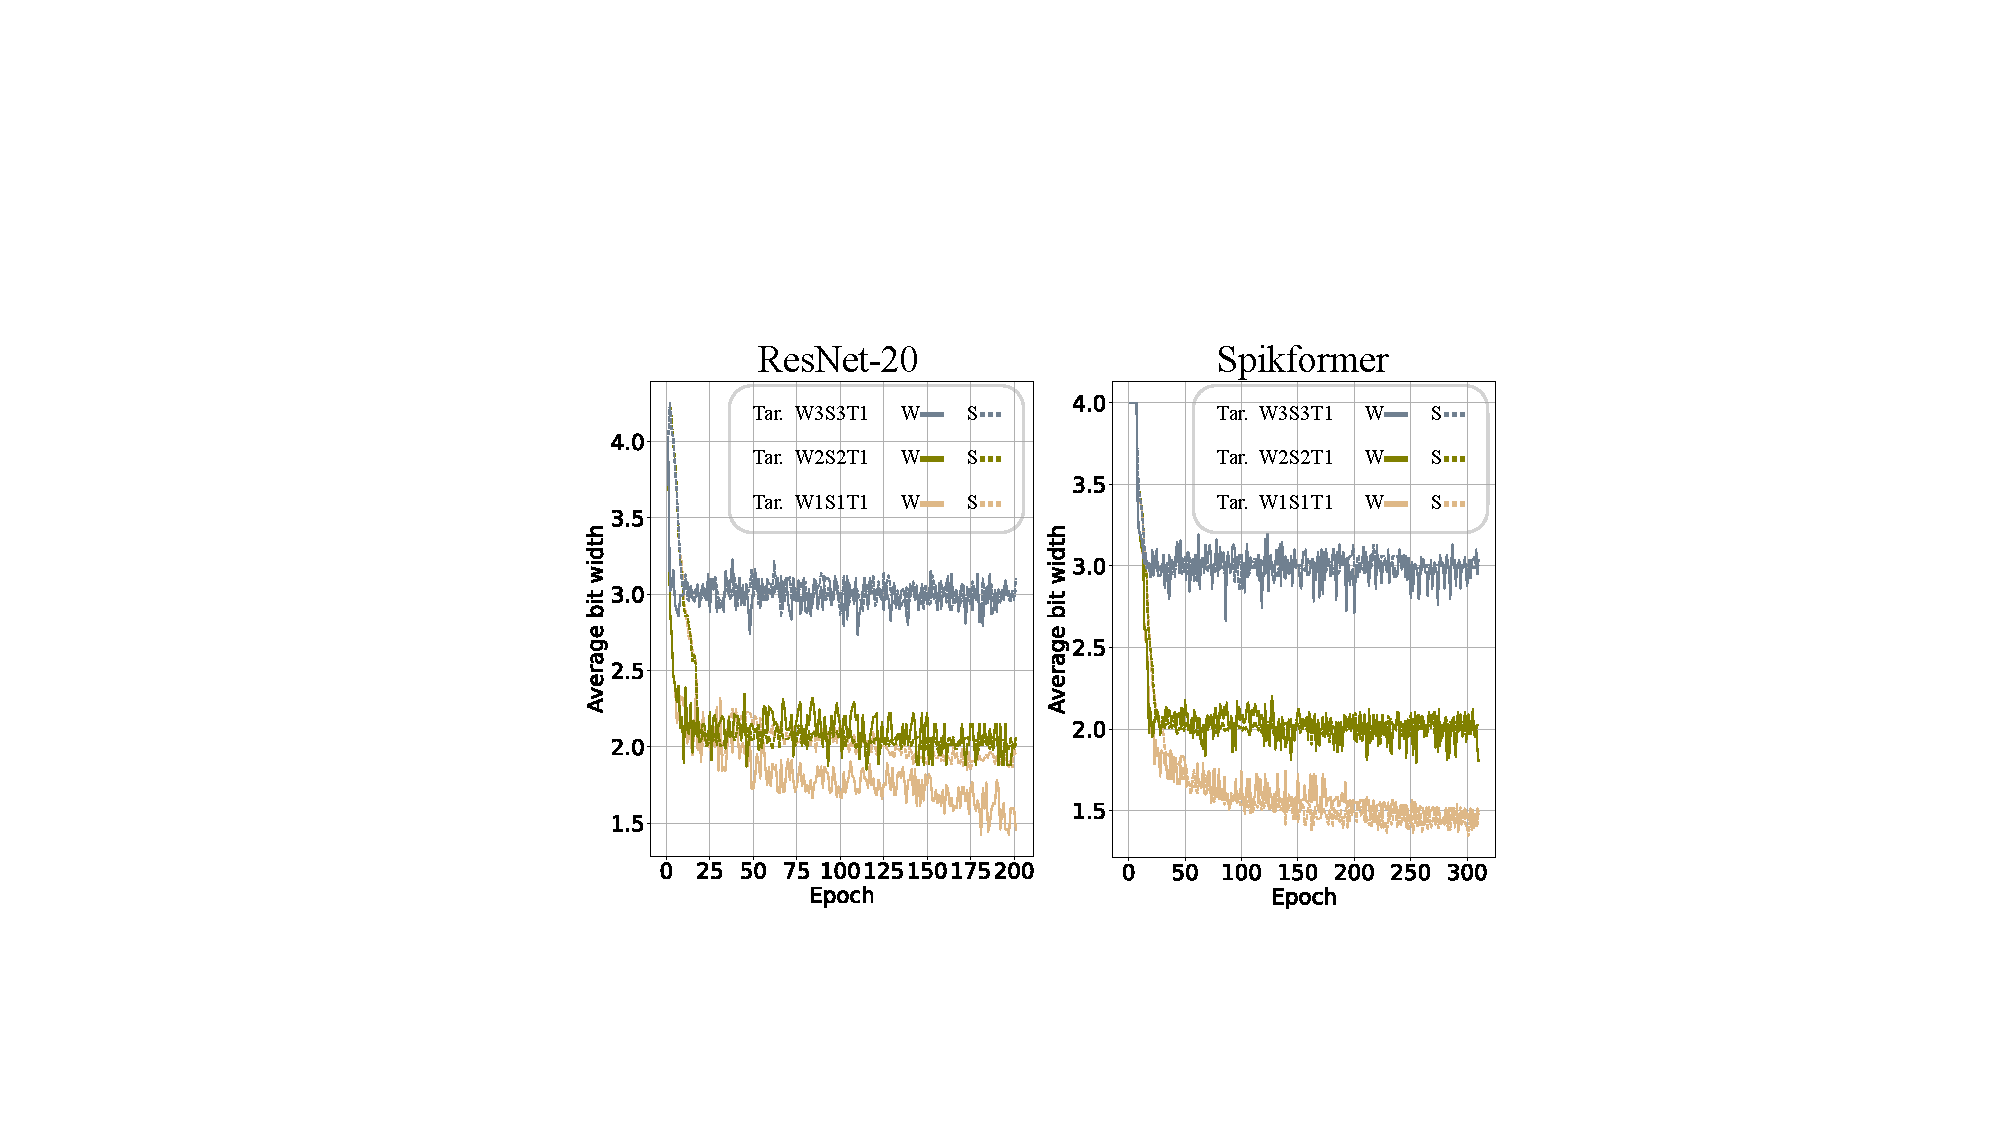
\includegraphics[width= 8cm]{figs/bit detect.pdf}
  \caption{Average bit width changes of ResNet-20 and Spikformer on CIFAR-10 during the adaptive-bit-width training. Tar. abbreviates target bit width. W, S, and T are weight, spike, and temporal bit width, respectively.
  }
  \label{fig:bit detect}
\end{figure}
\\\textbf{Step size renew mechanism.} To alleviate mismatch issue, we propose the following step-size renew mechanism. 
As illustrated in  \cref{fig:overview},
the renew mechanism is based on a bit width observer that watches on the bit width $B_l$, \eg, $B_{w,l}$ and $B_{s,l}$, and records the running maximum $V_{r\_max}$ and minimum $V_{r\_min}$ of the  data to be quantized. $V_{r\_max}$ and $V_{r\_min}$, reflecting the overall data distribution, will be used to renew the step size $S_l$, \eg, $S_q^l$ and $V_{th,l}^1$, directly.


Once $B_l$ is changed, the new $B_l$ will be recorded, the new $q_{max}$ and $q_{max}$ are calculated accordingly, and the observer will also instantly read the current maximum $V_{max}$ and minimum $V_{min}$ of the current batch of data $X$, \eg, weight or activation. 
Based on $V_{max}$ and $V_{min}$, a grid search is performed to calculate the currently optimal maximum $V'_{max}$ and minimum $V'_{min}$  as written in  \cref{algo:grid search}.  Finally, the running maximum $V_{r\_max}$ and minimum $V_{r\_min}$ are updated via 
\begin{equation}
\begin{split}
    &V_{r\_min} = min(V'_{min},V_{r\_min}),\\&V_{r\_max} = max(V'_{max},V_{r\_max}). 
\end{split}
\end{equation}
And, the renewed step size $S_l$ is determined via
\begin{align}
    S_l=\frac{V_{r\_max}-V_{r\_min}}{q_{max}-q_{min}}.
\end{align}

Thus, an optimal $S_l$ can be applied and cover the original one to correct the current forward pass. 
Since the grid search process will consume extra training time, we only activate the renew mechanism in the drastic bit reduction stage. Based on the observations of  \cref{fig:bit detect}, bit reduction mainly occurs in the first 12.5\% epochs. Therefore, we set a shutting threshold that once the difference between the current and the target bit width is below 24\% of the initial difference, the renew mechanism would be deactivated. Consequently, the training time increased by the grid search is lower than 0.05\% of the total training time.

% \begin{figure}[t]
%   \centering
%   \includegraphics[width= 8cm]{figs/reparam_spike_neuron.pdf}
%   \caption{Average bit width changes of ResNet-20 and Spikformer on CIFAR-10 during the adaptive-bit-width training. Tar. abbreviates target bit width, W is weight bit width, and S is the spike bit width.}
%   \label{fig:bit detect}
% \end{figure}


\begin{algorithm}[t]
	% \textsl{}\setstretch{1.8}
	\renewcommand{\algorithmicrequire}{\textbf{Input:}}
	\renewcommand{\algorithmicensure}{\textbf{Output:}}
    \caption{Grid search on $V_{max}$ and $V_{min}$.}
    \label{algo:grid search}
    \begin{algorithmic}[1]
		\REQUIRE Data to be quantized $X$, the $V_{max}$ and $V_{min}$ of $X$, the iteration number $K$, $q_{min}$, $q_{max}$, and the power constant $pow$.
  
		\ENSURE The optimal $V'_{max}$ and $V'_{min}$.

        \STATE $Score\gets 0$, $R\gets V_{max}-V_{min}$, $V'_{max} \gets V_{max}$, and $V'_{min} \gets V_{min}$.

        \STATE for $k=1; k\le K; i++$ do

        \STATE    \quad $V_{max}\gets \frac{k\cdot R}{K} $
        \STATE    \quad if $any(X<0)$ do
        \STATE    \quad \quad $V_{min}\gets -\frac{k\cdot R}{K} $
        \STATE    \quad else do
        \STATE    \quad \quad $V_{min}\gets 0 $
        \STATE  \quad $S'_l\gets\frac{V_{max}-V_{min}}{q_{max}-q_{min}}$ 

        \STATE  \quad $X_{q,k}\gets S'_l\cdot  clip(\left\lfloor\frac{X}{S'_l}\right\rceil,q_{min},q_{max})$
        \STATE  \quad $Score' \gets mean(|X_{q,k}-X|^{pow}) $
        \STATE  \quad if $Score' < Score$ do
        \STATE  \quad \quad $Score\gets Score'$
        \STATE  \quad \quad $V'_{max} \gets V_{max}$ and $V'_{min} \gets V_{min}$
        
    \end{algorithmic}$mean(x)$ is the element-wise averaging function. $any(x)$ checks if at least one element is True.
\end{algorithm}


\begin{table*}[t]
\centering
\caption{Comparisons with existing works on CIFAR. W/S/T denotes the averaged weight/spike/temporal bit width. Our models are initial to W/S/T=4/4/2.}
\label{tab:comparison on cifar}
\begin{adjustbox}{max width=0.9\textwidth}
\begin{threeparttable}
\begin{tabular}{cccccccccc}
\toprule
\multirow{2}{*}{\textbf{Method}} & \multirow{2}{*}{\textbf{Architecture}} & \multicolumn{4}{c}{\textbf{CIFAR 10}}                                                 & \multicolumn{4}{c}{\textbf{CIFAR 100}}                                        \\ \cmidrule(r){3-6} \cmidrule(r){7-10}                                  &                                        & \textbf{W/S/T}       & \textbf{Bit Budget} & \textbf{S-ACE (G)}          & \textbf{Top-1} & \textbf{W/S/T}          & \textbf{Bit Budget} & \textbf{S-ACE (G)}          & \textbf{Top-1} \\ \midrule
\multirow{2}{*}{Dspike \cite{li2021differentiable} }         & \multirow{2}{*}{ResNet20}     & 16/1/2               & 32            & 82.56          & 93.13          & 16/1/2         & 32         & 82.56          & 71.68          \\
                                 &                               & 16/1/4               & 64            & 165.58         & 93.66          & 16/1/4         & 64         & 165.58         & 73.35          \\ 
MLF \cite{fengmulti}                              & ResNet20                      & 16/1/4               & 64            & 165.58         & 94.25          & 16/1/4         & 64         & 165.58         & -              \\ 
\multirow{2}{*}{tdBN \cite{zheng2021going}}           & \multirow{2}{*}{ResNet19}     & 16/1/2               & 32            & 73.28          & 92.34          & 16/1/2         & 32         & 73.28          & -              \\
                                 &                               & 16/1/4               & 64            & 146.56         & 92.92          & 16/1/4         & 64         & 146.56         & -              \\ 
\multirow{2}{*}{TET \cite{deng2021temporal}}           & \multirow{2}{*}{ResNet19}     & 16/1/2               & 32            & 73.28          & 94.16          & 16/1/2         & 32         & 73.28          & 72.87          \\
                                 &                               & 16/1/4               & 64            & 165.12         & 94.44          & 16/1/4         & 64         & 165.12         & 74.47          \\ \midrule
\multirow{3}{*}{Ternary Spike \cite{guo2024ternary}}   & ResNet19                      & 16/2/1               & 32            & 330.24         & 95.58          & 16/2/1         & 32         & 330.24         & 78.45          \\ \cmidrule{2-10} 
                                 & \multirow{2}{*}{ResNet20}     & 16/2/2               & 64            & 165.58         & 94.48          & 16/2/2         & 64         & 165.58         & 73.41          \\
                                 &                               & 16/2/4               & 64            & 330.24         & 94.96          & 16/2/4         & 64         & 330.24         & 74.02          \\ \midrule
\multirow{3}{*}{Multi-bit Spike \cite{xiao2024multi}} & \multirow{3}{*}{ResNet20}     & 16/4/1               & 64            & 165.58         & 94.59          & 16/4/1         & 64         & 165.58         & 75.43          \\
                                 &                               & 16/4/4               & 256           & 660.48         & 94.93          & 16/4/4         & 256        & 660.48         & 76.51          \\
                                 &                               & 16/4/6               & 384           & 990.72         & 95.00          & 16/4/6         & 384        & 990.72         & -              \\ \midrule
\multirow{2}{*}{U-Quant.$\dagger$} & \multirow{2}{*}{ResNet20}     & 4/4/1                & 16            & 41.40          & 96.35          & 4/4/1          & 16         & 41.40          & 79.83          \\
                                 &                               & 4/4/2                & 32            & 82.79          & 96.39          & 4/4/2          & 32         & 82.79          & 80.19          \\ \midrule
Ours-111                         & \multirow{3}{*}{ResNet20}     & \textbf{1.38/1.32/1} & \textbf{1.83}  & \textbf{7.55}           & 96.15          & \textbf{2.06/1.58/3.25} & \textbf{3.25}  & \textbf{13.37}                   & 79.90          \\
Ours-222                         &                               & \textbf{2.13/2/2.08} & \textbf{8.87}  & \textbf{29.75 / 15.93*} & \textbf{96.48} & \textbf{2.11/1.98/2.08} & \textbf{8.66}  & \textbf{32.67 / 18.83*} & \textbf{80.59} \\
Ours-341                         &                               & \textbf{3.01/4.0/1}  & \textbf{12.08} & \textbf{39.49}          & \textbf{97.02} & \textbf{2.88/4.04/1}    & \textbf{11.64} & \textbf{40.60}          & \textbf{81.30}\\ \bottomrule         
\end{tabular}
\begin{tablenotes}
\footnotesize
\item $\dagger$ denotes plain uniform quantization, following  \cite{shen2024conventional}. $*$ denotes the temporal squeezing is applied in inference.  “Ours-xxx” denotes the target bit width of W/S/T.
\end{tablenotes}
\end{threeparttable}
\end{adjustbox}
\end{table*}

\begin{table}[t]
\centering
\caption{Comparisons with existing works on ImageNet.}
\label{tab:comparison on imagenet}
\begin{adjustbox}{max width=0.48\textwidth}
\begin{threeparttable}
\begin{tabular}{cccccc}
\toprule
\textbf{Method} & \textbf{Architecture}         & \textbf{W/S/T}         & \textbf{Bit Budget} & \textbf{S-ACE} & \textbf{Top-1} \\ \midrule
Hybrid training \cite{rathi2020enabling} & ResNet34                      & 16/1/250               & 4000                & 13608          & 61.48          \\
Spiking ResNet \cite{hu2021spiking}  & ResNet50                      & 16/1/350               & 5600                & 18952          & 72.75          \\
tdBN \cite{zheng2021going}           & ResNet34                      & 16/1/6                 & 96                  & 326.60         & 63.72          \\
Dspike \cite{li2021differentiable}         & ResNet34                      & 16/1/6                 & 96                  & 326.60         & 68.19          \\
MS-ResNet \cite{hu2024advancing}       & ResNet34                      & 16/1/6                 & 96                  & 326.60         & 69.42          \\ \midrule
TET \cite{deng2021temporal}             & Sew-ResNet34                  & 16/1/4                 & 64                  & 217.72         & 68.00          \\
Ternary Spike \cite{guo2024ternary}   & ResNet34                      & 16/2/4                 & 128                 & 435.47         & 70.74          \\ 
\multirow{2}{*}{PLIF+SEW \cite{fang2021deep}}     & SEW-ResNet34                  & 16/1/4                 & 64                  & 217.72         & 67.04          \\ 
                & SEW-ResNet50                  & 16/1/4                 & 64                  & 215.62         & 67.78          \\ 
Quant. SNN \cite{shen2024conventional}      & SEW-ResNet34                  & 8/8/1                  & 64                  & 217            & 70.13          \\ \midrule
Ours-221        & \multirow{3}{*}{SEW-ResNet34} & \textbf{2.58/2.18/1.0} & \textbf{5.61}      & \textbf{30.74} & 70.57 \\
Ours-241        &                               & \textbf{2.62/3.96/1.0} & \textbf{10.39}      & \textbf{54.69} & \textbf{72.02} \\
Ours-441        &                               & \textbf{3.93/3.92/1.0} & \textbf{15.4}      & \textbf{77.78} & \textbf{72.82} \\ \bottomrule
\end{tabular}

% \begin{tablenotes}
% \footnotesize
% \item $\dagger$ denotes plain uniform quantization, following  \cite{shen2024conventional}.
% \item $*$ denotes the temporal squeezing is applied in inference.
% \end{tablenotes}
\end{threeparttable}
\end{adjustbox}
\end{table}
\section{Experiments}
\label{sec:experiments}
In this section, we demonstrate our method's effectiveness. We first compare our results with the SoTA works using the ResNet architectures on CIFAR \cite{krizhevsky2009learning} and ImageNet-1k \cite{deng2009imagenet}, then
conduct ablation studies to verify different aspects of our method, including \textbf{(1)} each proposed technology's verification, \textbf{(2)} our method's extension to spiking self-attention \cite{zhou2022spikformer}, \textbf{(3)} conquering the “temporal constraint” of the prior arts \cite{shen2024conventional} on the event dataset CIFAR10-DVS \cite{li2017cifar10}, and \textbf{(4)} the learned bit allocation's visualization. \emph{All Implementation Details Are Attached in the Appendix.} 

\subsection{Comparisons with existing works}
\label{sbsec:comparison}
\textbf{CIFAR.} We apply our method to ResNet20 \cite{guo2024ternary} to compete with the SoTA SNNs. As shown in  \cref{tab:comparison on cifar}, we first compare our method with those learning- or module-based model optimization, \eg,  \cite{li2021differentiable, deng2021temporal, zheng2021going}, to prove our solution of non-differentiable terms performs well. Then, we compare with multi-bit SNNs, \eg,  \cite{guo2024ternary,xiao2024multi}, to prove we can achieve higher accuracy while using much lower memory (bit budget) and computation (S-ACE). Finally, compared with plain uniform quantization, our work can further squeeze the model accuracy to its limit while maintain lower memory and computation overhead, proving the effectiveness of adaptive bit allocation. Additionally, since we adopt the temporal squeezing technique as shown in  \cref{eq:our sn1} and  \cref{fig:overview}, the temporal dimension could also be compressed to 1 timestep before performing convolution, making sequential processing of SNNs more efficient during inference. That's why in the case of “W/S/T=222”, S-ACE can be further decreased. More elaborations on this are deferred to the appendix for better understanding.
\\\textbf{ImageNet.} We further apply our method to SEW-ResNet34 to demonstrate the superiority on the up-scaled dataset. As listed in  \cref{tab:comparison on imagenet}, compared with those using improved learning techniques or special modules  \cite{rathi2020enabling, zheng2021going,li2021differentiable,hu2024advancing}, we can achieve magnitudes of memory and computation savings without using any of their tricks. Furthermore, we can save 91.2\% memory (5.61 \vs64) and  85.83\% computation (30.74 \vs217) while achieve a higher accuracy (70.57\% \vs70.13\%) when compared with the quantized SNN. As bit budget increases, we can push accuracy to the advanced 72.82\% while still maintain lower memory and computation overhead, outperforming full-precision SNNs  \cite{guo2024ternary, fang2021deep, deng2021temporal}.

\subsection{Ablation study}
\label{sbsec:ablation}
We first continue to use ResNet20 and CIFAR10 to conduct ablation studies on the proposed techniques. Then, we migrate the proposed method to a different architecture Spikformer \cite{zhou2022spikformer} to further verify  effectiveness. On the extension to the event dataset, we push our method to conquer the “temporal constraint” issue, which doubles the prior art \cite{shen2024conventional}. 
Finally, we visualize the learned bit allocation. 
\\\textbf{Effectiveness of learnable bit width and the renew mechanism.} 
We first perform the plain uniform quantization (U-quant.) as the baselines, following  \cite{shen2024conventional}. As shown in \cref{exp:ablation on learnable bit}, the proposed learnable bit width technology (LBW) consistently outperforms U-quant, managing to allocate correct bit widths to different layers and improving the model accuracy to a higher level. Furthermore, we add the proposed renew mechanism only to the spike activation ($V_{th,l}^1$, Act.-only), or only to the weight ($S_q^l$, Weight-only), or to the bilateral case ($V_{th,l}^1$ and $S_q^l$). The results coherently show the renew mechanism can further improve LBW outcomes, mitigating the step-size mismatch issue.
As illustrated before, SNN would severely  suffer from the additional temporal quantization error. That's why Act.-only renew alone is effective enough to produce the best results. Bilateral renew seconds due to  a slightly lower bit budget. For simplicity, we adopt \emph{the 
Act.-only renew as the main method by default}.
\begin{table}[t]
\centering
\caption{Ablations on learnable bit width (LBW) and the renew mechanism. Different fonts denote the \textbf{1st}, the 
{\color[HTML]{9B9B9B} \textbf{2nd}}, and the  {\ul 3rd} best results, respectively. LBW models are initial to W/S/T=4/4/2.}
\label{exp:ablation on learnable bit}
\begin{adjustbox}{max width=0.49\textwidth}
\begin{threeparttable}
\begin{tabular}{c|c|cc||cc|cc|cc}
\toprule
\textbf{Target}         & \textbf{U-quant.} & \multicolumn{2}{c||}{\textbf{LBW}} & \multicolumn{2}{c|}{\textbf{\begin{tabular}[c]{@{}c@{}}LBW\\ +Weight-only Renew\end{tabular}}} & \multicolumn{2}{c|}{\textbf{\begin{tabular}[c]{@{}c@{}}LBW\\ +Bilateral Renew\end{tabular}}} & \multicolumn{2}{c}{\textbf{\begin{tabular}[c]{@{}c@{}}LBW\\ +Act.-only Renew\end{tabular}}} \\ \midrule
\textbf{W/S/T} & \textbf{Top-1}    & \textbf{W/S/T}  & \textbf{Top-1}  & \textbf{W/S/T}                                 & \textbf{Top-1}                                & \textbf{W/S/T}                    & \textbf{Top-1}                                           & \textbf{W/S/T}                    & \textbf{Top-1}                                          \\ \midrule
1/1/1          & 74.82             & 1.60/1.91/1.0   & {\ul 95.65}     & 1.73/1.98/1.0                                  & 93.28                                         & 1.25/1.36/1.0                     & {\color[HTML]{9B9B9B} \textbf{95.84}}                    & 1.38/1.32/1.0                     & {\color[HTML]{000000} \textbf{96.15}}                   \\
1/2/1          & 86.8              & 1.48/2.00/1.0   & {\ul 95.55}     & 1.57/2.12/1.0                                  & 93.52                                         & 1.25/2.04/1.0                     & {\color[HTML]{9B9B9B} \textbf{96.25}}                    & 1.42/2.08/1.0                     & \textbf{96.58}                                          \\
2/2/1          & 88.65             & 1.88/2.06/1.0   & 94.62           & 1.99/2.06/1.0                                  & {\ul 95.71}                                   & 2.00/1.89/1.0                     & {\color[HTML]{9B9B9B} \textbf{96.47}}                    & 2.08/2.08/1.0                     & \textbf{96.51}                                          \\
2/3/1          & 93.64             & 2.10/3.00/1.0   & 96.37           & 1.96/3.00/1.0                                  & {\ul 96.51}                                   & 2.02/3.06/1.0                     & {  \textbf{96.97}}                    & 2.24/3.06/1.0                     & {\color[HTML]{9B9B9B} \textbf{96.63}}                   \\
3/3/1          & 95.38             & 3.01/2.95/1.0   & 96.34           & 3.00/3.06/1.0                                  & {\ul 96.66}                                   & 2.87/3.04/1.0                     & {\color[HTML]{9B9B9B} \textbf{96.77}}                    & 2.89/2.87/1.0                     & \textbf{96.90}                                          \\
3/4/1          & 96.09             & 2.87/4.10/1.0   & 96.72           & 2.90/3.98/1.0                                  & {\ul 96.89}                                   & 2.97/3.94/1.0                     & {\color[HTML]{9B9B9B} \textbf{97.01}}                    & 3.01/4.00/1.0                     & \textbf{97.02}                                          \\
4/4/1          & 96.35             & 4.04/4.06/1.0   & 96.78           & 3.99/4.02/1.0                                  & {\ul 97.00}                                   & 3.86/4.00/1.0                     & {\color[HTML]{9B9B9B} \textbf{97.03}}                    & 3.99/4.06/1.0                     & \textbf{97.05}                                          \\
4/4/2          & 96.39             & 4.02/3.93/1.92  & {\ul 96.80}     & 3.88/4.04/2.0                                  & 96.57                                         & 4.01/3.97/2.0                     & {  \textbf{97.03}}                    & 3.93/4.03/2.08                    & {\color[HTML]{9B9B9B} \textbf{96.92}}                   \\ \bottomrule
\end{tabular}
% \begin{tablenotes}
% \footnotesize
% \item $\dagger$ denotes plain uniform quantization, following  \cite{shen2024conventional}.
% \item $*$ denotes the temporal squeezing is applied in inference.
% \end{tablenotes}
\end{threeparttable}
\end{adjustbox}
\end{table}
\begin{table}[t]
\centering
\caption{Ablations on the refined spiking neuron. Different fonts denote the \textbf{1st}, the 
{\color[HTML]{9B9B9B} \textbf{2nd}}, and the  {\ul 3rd} best results, respectively.}
\label{exp:ablation on refined neuron}
\begin{adjustbox}{max width=0.48\textwidth}
\begin{threeparttable}
\begin{tabular}{c|c|cc|cc|cc|cc}
\toprule
{  \textbf{Target} }                                                                                  & {  \textbf{\begin{tabular}[c]{@{}c@{}}$\tau=2$\& \cref{eq:mlif3} \\ U-quant.\end{tabular}}} & \multicolumn{2}{c|}{{  \textbf{\begin{tabular}[c]{@{}c@{}}$\tau=2$\& \cref{eq:mlif3}  \\ w/o renew\end{tabular}}}} & \multicolumn{2}{c|}{{  \textbf{\begin{tabular}[c]{@{}c@{}}$\tau=2$\& \cref{eq:mlif3} \\ w/ renew\end{tabular}}}} & \multicolumn{2}{c|}{{  \textbf{\begin{tabular}[c]{@{}c@{}}$\tau=2$\& \cref{eq:our sn3}\\ w/ renew\end{tabular}}}} & \multicolumn{2}{c}{{  \textbf{\begin{tabular}[c]{@{}c@{}}$\tau=1$\& \cref{eq:our sn3}\\ w/ renew\end{tabular}}}} \\ \midrule
{  \textbf{ W/S/T}} & {  \textbf{Top-1}}                                                       & {  \textbf{W/S/T}}                    & {  \textbf{Top-1}}                   & {  \textbf{W/S/T}}                   & {  \textbf{Top-1}}                  & {  \textbf{W/S/T}}                   & {  \textbf{Top-1}}                  & {  \textbf{W/S/T}}                  & {  \textbf{Top-1}}                  \\ \midrule
{  1/1/1}                                                                              & {  74.82}                                                                & {  1.80/2.14/1.0}                     & {  95.12}                            & {  1.80/2.09/1.0}                    & {  {\ul 95.58}}                     & {  1.46/1.34/1.0}                    & {\color[HTML]{9B9B9B} \textbf{95.71}}                  & {  1.38/1.32/1.0}                   & {  \textbf{96.15}}                  \\
{  1/2/1}                                                                              & {  10.02}                                                                & {  1.77/2.2/1.0}                      & {  95.21}                            & {  1.58/2.13/1.0}                    & {  {\ul 96.14}}                     & {  1.40/2.05/1.0}                    & {\color[HTML]{9B9B9B} \textbf{96.48}}                  & {  1.42/2.08/1.0}                   & {  \textbf{96.58}}                  \\
{  2/2/1}                                                                              & {  0.1}                                                                  & {  2.10/2.07/1.0}                     & {  95.50}                            & {  2.09/1.97/1.0}                    & {  {\ul 96.04}}                     & {  1.88/1.95/1.0}                    & {\color[HTML]{9B9B9B} \textbf{96.45}}                  & {  2.08/2.08/1.0}                   & {  \textbf{96.51}}                  \\
{  2/3/1}                                                                              & {  89.06}                                                                & {  2.05/3.01/1.0}                     & {  {\ul 96.51}}                      & {  2.13/3.16/1.0}                    & {  96.38}                           & {  1.96/3.04/1.0}                    & {  \textbf{96.72}}                  & {  2.24/3.06/1.0}                   & {\color[HTML]{9B9B9B} \textbf{96.63}}                  \\
{  3/3/1}                                                                              & {  0.1}                                                                  & {  2.98/3.02/1.0}                     & {  96.18}                            & {  3.01/3.07/1.0}                    & {  {\ul 96.43}}                     & {  3.03/3.01/1.0}                    & {\color[HTML]{9B9B9B} \textbf{96.82}}                  & {  2.89/2.87/1.0}                   & {  \textbf{96.90}}                  \\
{  3/4/1}                                                                              & {  96.31}                                                                & {  3.06/3.98/1.0}                     & {  96.64}                            & {  2.99/4.02/1.0}                    & {  {\ul 96.80}}                     & {  2.95/4.06/1.0}                    & {\color[HTML]{9B9B9B} \textbf{97.00}}                  & {  3.01/4.0/1.0}                    & {  \textbf{97.02}}                  \\ \bottomrule
\end{tabular}
% \begin{tablenotes}
% \footnotesize
% \item $\dagger$ denotes plain uniform quantization, following  \cite{shen2024conventional}.
% \item $*$ denotes the temporal squeezing is applied in inference.
% \end{tablenotes}
\end{threeparttable}
\end{adjustbox}
\end{table}
\begin{table}[b]
\centering
\caption{Ablations of Spikformer-4-384 on CIFAR10. Different fonts denote the \textbf{1st} and the 
{\color[HTML]{9B9B9B} \textbf{2nd}} best results, respectively.}
\label{exp:ablation of spf}
\begin{adjustbox}{max width=0.46\textwidth}
\begin{threeparttable}
\begin{tabular}{c|c|cc|cc|cc}
\toprule
{ \textbf{ Target }}                                                                                   & {  \textbf{U-quant.}} & \multicolumn{2}{c|}{{  \textbf{LBW}}}                & \multicolumn{2}{c|}{{  \textbf{LBW + renew}}}                 & \multicolumn{2}{c}{\textbf{Origin \cite{zhou2022spikformer}}}          \\ \midrule
{  \textbf{W/S/T}} & {  \textbf{Top-1}}    & {  \textbf{W/S/T}} & {  \textbf{Top-1}} & {  \textbf{W/S/T}} & {  \textbf{Top-1}} & \textbf{W/S/T}           & Top-1                   \\ \midrule
{  1/1/1}                                                                              & {  79.53}             & {  1.44/1.48/1.0}  & {\color[HTML]{9B9B9B} \textbf{95.37}} & {  1.53/1.5/1.0}   & {  \textbf{95.47}} &                          &                         \\
{  1/2/1}                                                                              & {  89.3}              & {  1.47/1.99/1.0}  & {  \textbf{95.68}} & {  1.47/2.01/1.0}  & {\color[HTML]{9B9B9B} \textbf{95.54}} &                          &                         \\
{  2/2/1}                                                                              & {  89.68}             & {  1.88/2.03/1.0}  & {\color[HTML]{9B9B9B} \textbf{95.80}} & {  2.02/2.01/1.0}  & {  \textbf{95.84}} &                          &                         \\
{  2/3/1}                                                                              & {  94.11}             & {  2.00/2.94/1.0}  & {\color[HTML]{9B9B9B} \textbf{95.93}} & {  2.15/2.95/1.0}  & {  \textbf{96.04}} &                          &                         \\
{  3/3/1}                                                                              & {  94.21}             & {  2.93/3.01/1.0}  & {\color[HTML]{9B9B9B} \textbf{95.87}} & {  2.89/2.99/1.0}  & {  \textbf{95.99}} & \multirow{-5}{*}{16/1/4} & \multirow{-5}{*}{95.19} \\ \bottomrule
\end{tabular}

% \begin{tablenotes}
% \footnotesize
% \item $\dagger$ denotes plain uniform quantization, following  \cite{shen2024conventional}.
% \item $*$ denotes the temporal squeezing is applied in inference.
% \end{tablenotes}
\end{threeparttable}
\end{adjustbox}
\end{table}
\\\textbf{Importance of the refined spiking neuron.}
We further verify the effectiveness of the refined spiking neuron. The major differences are that we refine  \cref{eq:mlif3} to  \cref{eq:our sn3} and suggest using the IF neuron rather than LIF, \ie, using $\tau=1$ rather than the default $\tau=2$ \cite{fang2023spikingjelly}. In  \cref{exp:ablation on refined neuron}, the results consistently show that the original multi-bit neuron would impair the quantized model's robustness, while our refining tricks and renew mechanism steadily improve the model performance to better states. Thus, enabling the advancement of high-performance and low-overhead SNNs. 
\begin{table}[t]
\centering
\caption{Spikformers on CIFAR10-DVS. The \textbf{best results} and {\ul temporal lengths} are highlighted.}
\label{exp:ablations on dvs}
\begin{adjustbox}{max width=0.45\textwidth}
\begin{threeparttable}
\begin{tabular}{cc|cc|cc}
\hline
\multicolumn{2}{c|}{\textbf{Origin} \cite{shen2024conventional}}             & \multicolumn{2}{c|}{\textbf{Quant. Spkiformer} \cite{shen2024conventional}} & \multicolumn{2}{c}{\textbf{Our Spkiformer}} \\ \hline
\textbf{W/S/T}           & \textbf{Top-1}        & \textbf{W/S/T}      & \textbf{Top-1}      & \textbf{W/S/T}    & \textbf{Top-1}    \\ \hline
\multirow{5}{*}{16/1/16} & \multirow{5}{*}{80.7} & 1/1/{\ul16}             & \textbf{79.8}       & 1.11/2.00/{\ul6.0}     & \textbf{80.9}     \\
                         &                       & 1/2/{\ul8}             & 79.3                & 1.28/2.00/{\ul4.0}     & 80.0              \\
                         &                       & 1/4/{\ul4}            & 63.1                & 1.33/4.00/{\ul3.0}     & 80.1              \\
                         &                       & 1/8/{\ul2}            & 43.0                & 1.31/4.03/{\ul2.0}     & 78.7              \\
                         &                       & 1/16/{\ul1}          & 35.8                & 1.31/4.03/{\ul1.0}     & 77.4              \\ \hline
\end{tabular}
% \begin{tablenotes}
% \footnotesize
% \item \textbf{TS} abbreviates temporal squeezing.
% \end{tablenotes}
\end{threeparttable}
\end{adjustbox}
\end{table}
\begin{figure}[b]
  \centering
  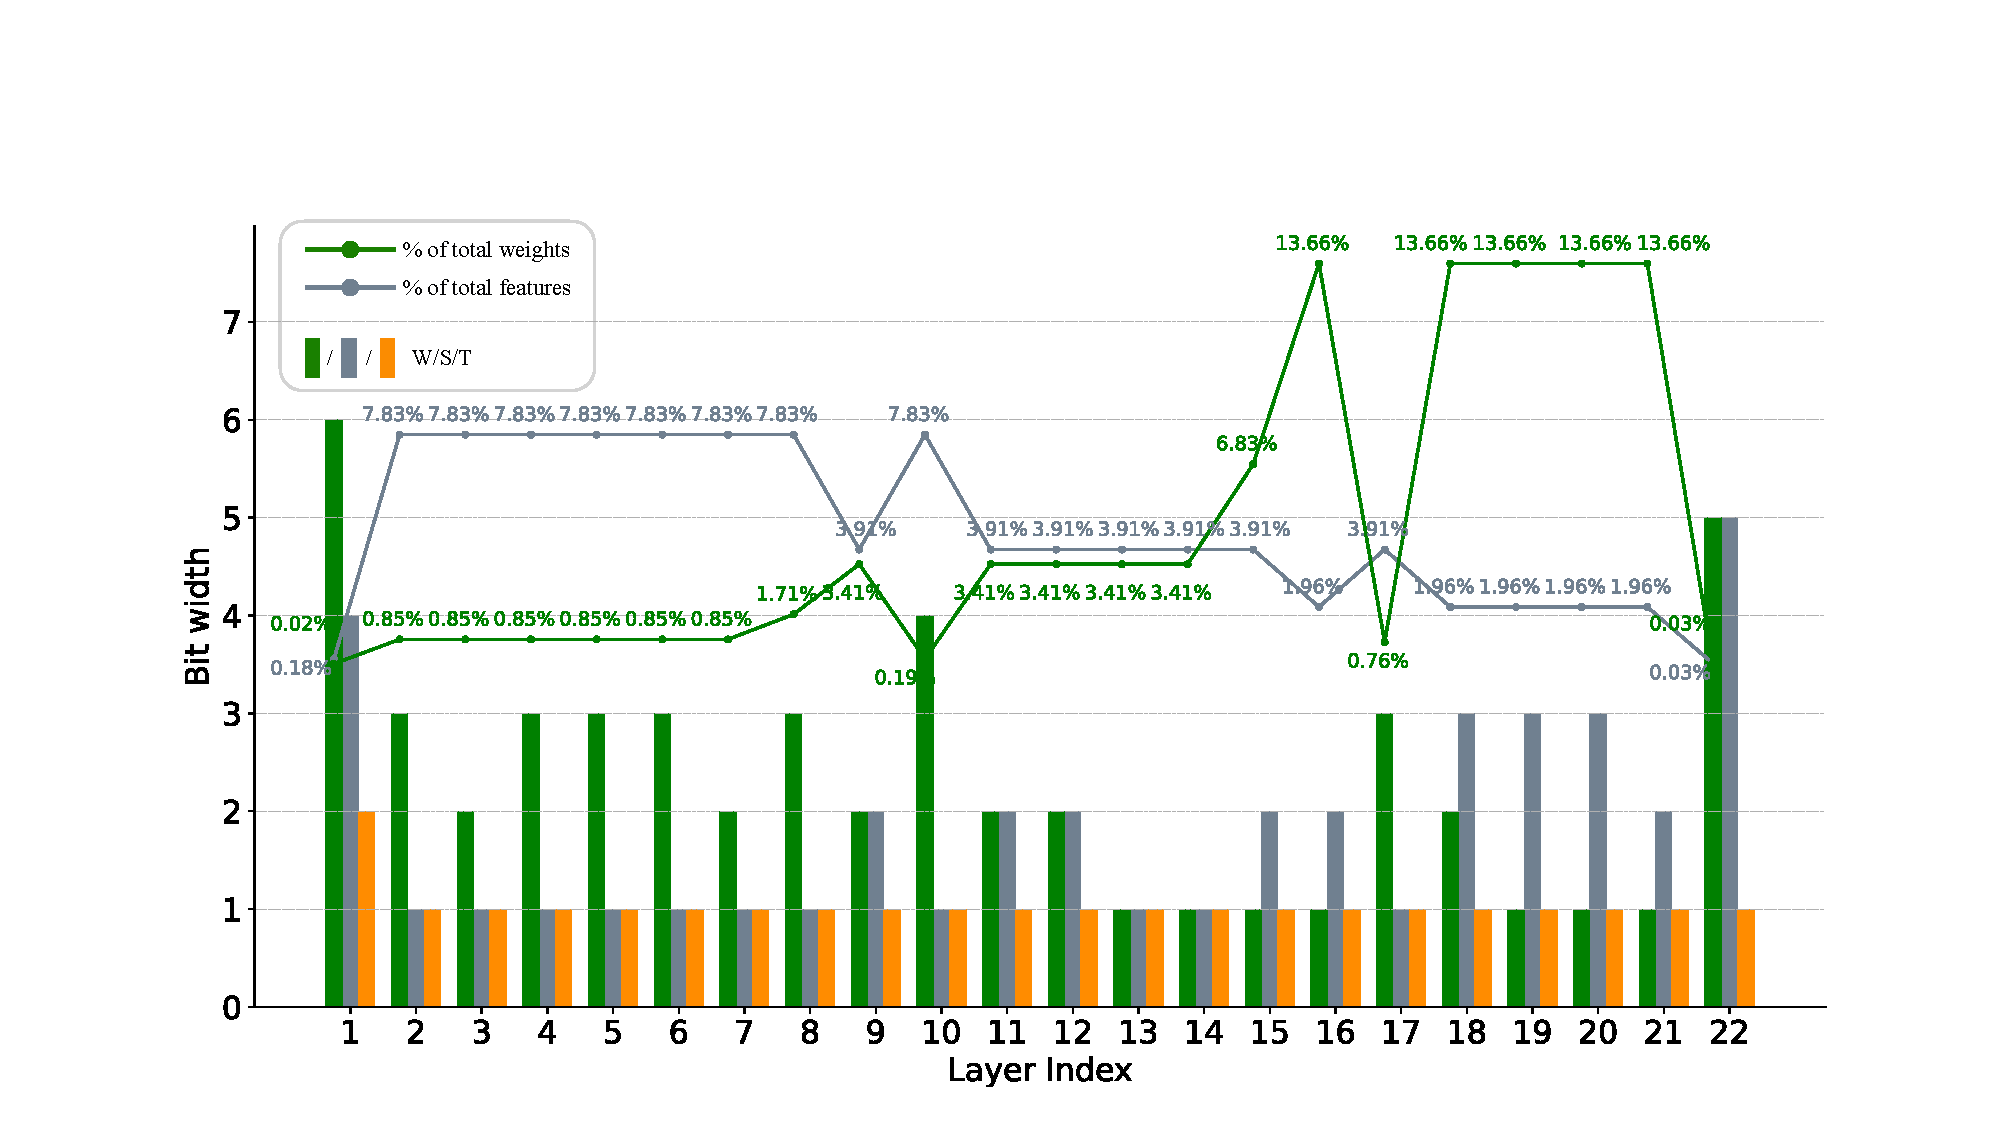
\includegraphics[width= 8cm]{figs/bit_vis.pdf}
  \caption{Statistics of each layer's bit widths. Since layer \#1 has two time-steps, we report the averaged spike bit width for clarity.}
  \label{fig:bit_vis}
\end{figure}
\\\textbf{Validation on spiking self-attention architectures.}
We then consider a new architecture Spikformer. Migrating our method to Spikformer is \textbf{non-trivial} because the self-attention operation is a different computing paradigm where a new quantizable tensor $atten$ arises. We would like to leave room for future work. Here, we naively apply our method to Spikformer as depicted in  \cref{fig:intro} to validate migratability.  We adopt the default Spikformer-4-384 \cite{zhou2022spikformer} on CIFAR10. As listed in  \cref{exp:ablation of spf}, with our LBW, the model accuracy surpasses the original Spikformer under the same hyperparameters, while plain quantization fails. Adding the the renew mechanism would further boost the performance.
\\\textbf{Conquering the temporal constraint.}
We further test the migratability on the special event dataset. We use the same default Spikformer and settings as  \cite{shen2024conventional} without any data augmentation. As shown in  \cref{exp:ablations on dvs}, “temporal constraint” refers to the dramatic accuracy decrease of event datasets as temporal length declines to the extremely low time-step \cite{shen2024conventional}. However, in our work, such phenomenon disappears and accuracy is well maintained even in the case of $T=1$. 
This implies that spatial information can be better extracted with our method even in the sparse event data.
Meanwhile, we are in line with prior findings that temporal information matters more than spatial information to event datasets. 
Moreover, compared with the original Spkiformer, our method can achieve higher accuracy with lower bit budgets
and time steps, proving the effectiveness on event data.
\\\textbf{Statistics of bit widths.} Last but not least, we visualize the learned bit allocation of ResNet20 with W/S/T = 1.38/1.32/1 on CIFAR10 to visually confirm effectiveness. Notably, different from any prior arts \cite{guo2024ternary,zheng2021going,fang2021deep}, we add additional spiking neurons before the first layer to fully benefit the model with addition-only computation. In consistence with the previous setting, the model is initialized to W/S/T = 4/4/2. 
As vividly displayed in  \cref{fig:bit_vis}, \textbf{(1)} the layers with the higher proportion of feature and weight tend to get lower bits thus lowering the overall memory and computation. \textbf{(2)} The 1st and last layers tend to learn higher bit widths, which is line with their outstanding importance as reported in prior arts \cite{choi2018pact}. With \textbf{(1)} and \textbf{(2)} combined, we conclude our adaptive bit allocation method should be sensible and effective.







% \begin{table}[t]
% \centering
% \caption{Comparisons with existing works on ImageNet.}
% \label{exp:comparison with ann baseline}
% \begin{adjustbox}{max width=0.48\textwidth}
% \begin{threeparttable}

% % \begin{tablenotes}
% % \footnotesize
% % \item $\dagger$ denotes plain uniform quantization, following  \cite{shen2024conventional}.
% % \item $*$ denotes the temporal squeezing is applied in inference.
% % \end{tablenotes}
% \end{threeparttable}
% \end{adjustbox}
% \end{table}

\section{Conclusion}
\label{sec:conclusion}
In this paper, we propose an adaptive bit allocation method, based on learnable bit widths, for efficient and accurate SNNs. 
To solve the new challenges brought by the special temporal dimension of SNN, we refine the spiking neuron to enable temporal matching inter- and intra-layer and increase the adaptivity via better neuron formulations for better model performance. We further theoretically formulate the step size mismatch issue that would temporally deteriorate, and alleviate it by the proposed renew mechanism.
Thorough experiments are conducted to prove every aspects is effective. 
Eventually, we advance accuracy with lower memory (Bit budget) and computation (S-ACE) overhead.


{
    \small
    \bibliographystyle{ieeenat_fullname}
    \bibliography{main}
}




% WARNING: do not forget to delete the supplementary pages from your submission 
% \clearpage
\setcounter{page}{1}
\maketitlesupplementary


\section{Rationale}
\label{sec:rationale}
% 
Having the supplementary compiled together with the main paper means that:
% 
\begin{itemize}
\item The supplementary can back-reference sections of the main paper, for example, we can refer to \cref{sec:intro};
\item The main paper can forward reference sub-sections within the supplementary explicitly (e.g. referring to a particular experiment); 
\item When submitted to arXiv, the supplementary will already included at the end of the paper.
\end{itemize}
% 
To split the supplementary pages from the main paper, you can use \href{https://support.apple.com/en-ca/guide/preview/prvw11793/mac#:~:text=Delete%20a%20page%20from%20a,or%20choose%20Edit%20%3E%20Delete).}{Preview (on macOS)}, \href{https://www.adobe.com/acrobat/how-to/delete-pages-from-pdf.html#:~:text=Choose%20%E2%80%9CTools%E2%80%9D%20%3E%20%E2%80%9COrganize,or%20pages%20from%20the%20file.}{Adobe Acrobat} (on all OSs), as well as \href{https://superuser.com/questions/517986/is-it-possible-to-delete-some-pages-of-a-pdf-document}{command line tools}.

\end{document}
